\documentclass[a4paper]{article}
\usepackage[T1]{fontenc}
\usepackage[utf8]{inputenc}
\usepackage[english]{babel}
\usepackage[bottom]{footmisc}
\usepackage{amsmath,amsfonts,amsthm}
\usepackage{geometry}
\geometry{a4paper, top=3cm, bottom=3cm, left=2cm, right=2cm}
\usepackage{comment}
\usepackage{graphicx}
\usepackage{caption}
\usepackage{subcaption}
\usepackage{float}
\usepackage{enumitem}
\usepackage{fourier}
%\usepackage{subfigure}


\usepackage[backend=biber]{biblatex}%,sorting=ydnt
\addbibresource{bib.bib}



\begin{comment}

%\title{\bf{Titolo}}
\title{%\vspace{2 cm} 

\begin{flushleft}
\begin{LARGE}
POPULATION DYNAMICS OF MULTI-SPECIES ECOLOGICAL SYSTEMS: STABILITY ANALYSIS\\\end{LARGE}
\vspace{0.5 cm}
\begin{large}
Physics of Complex Systems course project\\ \end{large}\vspace{0.3 cm}
\begin{LARGE}
Silvia Maria Macrì\\
\end{LARGE}
\end{flushleft}
}
\date{}
%\date{A.A. 2019/2020}
%\author{Silvia Maria Macrì 
%A.A. 2019/2020
%\vspace{3 cm}}
\end{comment}

\title{DEVELOPMENT OF A CLUSTERING ALGORITHM BASED ON THE MONDRIAN PROCESS\\
Models and Numerical Methods course project}
\date{}
\author{Silvia Maria Macrì} 




\begin{document}


\tableofcontents
\newpage



%facciamo così: per i modelli numerici sviluppa ed illustra le proprietà e le caratteristiche del processo di Mondrian utilizzato come classificatore: ovvero perchè funziona, come si implementa e le problematiche numeriche connesse alla metodologia con un esempio di applicazione. Fai un piccolo elaborato che illustri all'esame e poi ti farò una domando sul programma.









\maketitle


%\abstract

The scope of this report is to exploit the Mondrian process, a temporal stochastic process that hierarchically partitions the space, in order to develop an unsupervised method that classify unlabeled data.
After a brief remind of what cluster analysis is, the Mondrian process and some of its properties are illustrated;
then, a clustering algorithm based on the process is described.
Finally, some examples are shown, in order to highlight some methodological characteristics and issues related to the formulation of the process. 




%\tableofcontents



\section{Clustering}

Cluster analysis is a machine learning approach whose scope is to divide a population of data into a certain number of groups.
In contrast with supervised learning methods, like classification, in which data are grouped on the basis of some existing labeling, clustering deals with unlabeled data, and the division into classes is performed in order to maximize intra-class similarity and minimize inter-class similarity.
Since there is not an unique and precise definition of similarity, each clustering algorithm is characterized by a specific metric.
%The similarity measure that is used is a specific characteristic of each clustering algorithm.

The wide variety of clustering algorithms can be categorized in different ways;
a fundamental difference is, for example, between hierarchical and partition clustering approach.
The hierarchical clustering groups data by using top-down and bottom-up approach:
the divisive or top-down algorithms start to consider the whole set of data as belonging to an unique initial cluster, that is progressively divided into an increasing number of clusters, in order to maintain more homogeneous groups of data;
on the contrary, the aggregative or bottom-up algorithms start with each element of the set of data belonging to different clusters and progressively merges them until a specific condition is satisfied.  
The partition clustering doesn't have a hierarchical structure but assigns data into a certain number of clusters by progressively optimizing some criterion function.


\paragraph{Decision tree}

Given a set of data $X \subseteq \mathbb{R}^D$, a decision tree on $X$ can be defined as a hierarchical, axis-aligned, binary partitioning of $X$ \cite{2015MPMachineLearning}.
It has a network structure, where each node represents a specific restriction of the initial dataset.
%, created on the basis of some intrinsic characteristic of the data (the labeling in classification or the similarity criterion in clustering).
%This means that the space in which $X$ is defined is hierarchically divided into subsequent subspaces, and each division is performed on the basis of some characteristic of the data.
The binarity of the tree means that each non-leaf node is linked to exactly two children and, except for the root node that represents the whole data space $X$, each node has only one father;
in particular, the set of data corresponding to the father node splits into two subsets assigned respectively to the two children.
The term axis-aligned means that each split of a father into two children is performed by imposing a threshold value on only one of the features;
if we visualize the tree structure in a product space, this means that each cut is performed orthogonally to one of the axis.
The union of the subspaces corresponding to the leaf nodes coincides with the initial space $X$ and their intersection is an empty set.
%A characteristic of a binary decision tree applied to both supervised or unsupervised learning is that each classification of the data into groups is performed on a subset of the total amount of data $X$.
Because of its hierarchical structure, the decision tree can be used as hierarchical clustering method (with both top-down and bottom-up approach), by selecting a data-dependent splitting (or merging) criterion.


\section{The Mondrian Process}

\subsection{Definition}\label{defMP}

%The Mondrian process is defined as a temporal stochastic process taking values in the ensemble of\footnote{?} guillotine partitions of an axis-aligned box.
The Mondrian process is a recursive generative process, defined over an axis-aligned box $\Theta \subseteq \mathbb{R}^D$, that hierarchically partitions the underlying space through axis-aligned cuts \cite{2008MondrianProcess}. % some hyperplane orthogonal to one of the $D$ coordinate axes.
%A random variable X is a variable that may assume only the values of a given sample space S, with a given probability.
% A stochastic process is defined as a collection of indexed random variables defined on a common probability sample space
% lo spazio da dove vengono presi i valori è l'insieme di tutte le guillotine partitions su teta---> quindi è infinito
Given an axis-aligned box $\Theta = [a_1,b_1] \times \ldots \times [a_D,b_D] \subseteq \mathbb{R}^D$, defined as the cartesian product of bounded intervals, the process generates two subspaces $\Theta_<$ and $\Theta_>$ by splitting $\Theta$ with some hyperplane orthogonal to one of the coordinate axis; 
then, it similarly generates independent splits on $\Theta_<$ and $\Theta_>$, creating new subspaces that are recursively cut until a certain condition is satisfied.
%An axis-aligned box $\Theta = [a_1,b_1] \times \ldots \times [a_D,b_D] \subseteq \mathbb{R}^D$ is defined as the cartesian product of bounded intervals, 
%while a guillotine partition of $\Theta$ is a hierarchical partition of $\Theta$ obtained by recursively splitting the space through hyperplanes orthogonal to the coordinate axes.\footnote{ copiato}
%The following recursive generative process determines the temporal distribution of the cuts:\footnote{temporal distribution?}\\ \\
The following scheme shows the generative process in detail:\\ \\
MONDRIAN($\Theta$,$t_0$):
\begin{enumerate}[nolistsep]
\item $T \sim Exp(LD(\Theta))$ 
\item $d \sim$ Discrete$(p_1,...,p_D)$ where $p_d \propto (b_d-a_d)$
\item $x \sim \mathcal{U}([a_d,b_d])$
\item $M_< \leftarrow$ MONDRIAN($\Theta_<$,$t_0+T$) where $\Theta_< = \{\emph{z} \in \Theta \lvert z_d \leq x \}$ 
\item $M_> \leftarrow$ MONDRIAN($\Theta_>$,$t_0+T$) where $\Theta_> = \{\emph{z} \in \Theta \lvert z_d \geq x \}$ 
\end{enumerate}
return ($t_0+T,d,x,M_<,M_>$)\\ \\%t_0,\Theta_<,\Theta_>,


The process is initialized by fixing the starting time $t_0$ and the initial axis-aligned box $\Theta$ that will be partitioned.
Firstly, in line 1, the time $T$ of the first cut is randomly generated from an exponential distribution, with rate the linear dimension of the box $LD(\Theta) = \sum_{d=1}^D(b_d-a_d)$;
this means that cuts in smaller boxes are expected to occur later than in bigger ones.
The absolute time $t_0 +T$ at which the cut is generated is called birth time. 
Then, the dimension $d$ of the cut is generated from a discrete distribution, with a probability proportional to the length $b_d-a_d$ of the corresponding interval (line 2), and the location of the cut is subsequently uniformly chosen in the interval $[a_d,b_d]$ (line 3).\\
At this point, the initial space $\Theta$ has been cut by an hyperplane orthogonal to the d-dimension and intersecting the $[a_d,b_d]$ interval in $d=x$, and it has been divided into two axis-aligned boxes $\Theta^<$ and $\Theta^>$.
Lines 4 and 5 generate independent Mondrians on the two new subspaces, meaning that steps 1,2 and 3 are independently repeated on $\Theta_<$ and $\Theta_>$, starting from an initial time equal to the birth time of the last cut. \\
The process recursively splits the space in more and more refined partitions and stops when, for every independent Mondrian that has been generated, the birth time $t_0+T$ of the last cut is higher than a fixed lifetime parameter $\lambda$.
The lifetime $\lambda$ represents a budget assigned to the process and, as cuts appear, it is progressively spent;
it follows that the time interval $T$, that is generated at each iteration, represents the cost related to a specific cut.


\subsubsection*{The Mondrian process as temporal stochastic process}
The formulation of Mondrian process as recursive generative process leads to an other definition as temporal stochastic process.
More precisely, given an axis-aligned box $\Theta \subseteq \mathbb{R}^D$, the Mondrian process on $\Theta$, denoted as $MP(\Theta)$, can be defined as a temporal stochastic process $(M_t)_{t>0}$ taking values in the ensemble of guillotine partitions of $\Theta$ and with distribution specified by the generative process MONDRIAN($\Theta,t_0$) \cite{2015MPMachineLearning}.
If we define a guillotine partition as a hierarchical partition of $\Theta$ obtained by recursively splitting the space through hyperplanes orthogonal to the coordinate axes, the random variable $(M_t)_{t>0}$ is a %\footnote{the or a} 
guillotine partition of $\Theta$ formed by the cuts with birth time $t_b \leq t$.%\footnote{praticamente copiato}
%\footnote{definito nello spazio di tutte le possibili guillotine partition?}



\subsubsection*{Tree structure of the Mondrian process}

The hierarchical structure of Mondrian process reflects the structure of a rooted binary k-d tree;
each node is represented by the tuple ($t_0+T,d,x,M_<,M_>$), which entries are the birth time, the dimension and the location of the cut and the two children of the node itself.
Each non-leaf node has exactly two children and the ensemble of the leaf nodes represents the final and more refined partition of the initial space.
The lifetime parameter $\lambda$ of the stochastic process, that regulates the total number of cuts, can be interpreted as the depth parameter of the tree.



\begin{figure}[H]
        \centering
        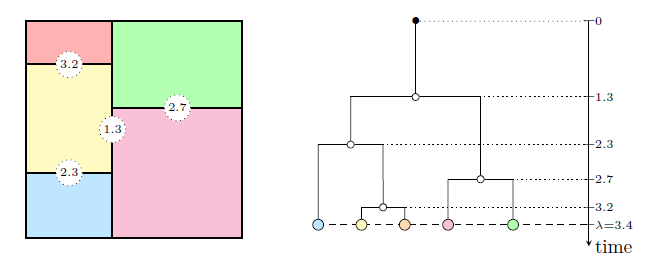
\includegraphics[width=10cm]{grafici/MP.png}
\caption{A Mondrian partition (left) with corresponding tree structure (right),
which shows the evolution of the tree over time \cite{mourtada2019minimax}}
        \label{MP}
    \end{figure}   






\subsection{Properties of the Mondrian process}



%per quanto riguarda la parte teorica su mondrian process, puoi evitare di parlare del processo di dirichlet se non lo capisci per l'esame


% distribuzione di poisson (discreta):
%indica la probabilità che accadano un certo numero di eventi in un intervallo di tempo
% il parametro indica il numero medio di eventi per intervallo di tempo
%if X and Y are independent Poisson random variables, then X +Y is also Poisson and the conditional distribution of X given X + Y is binomial

%\subsubsection*{MONDRIAN PROCESS AS MULTIDIMENSIONAL GENERALIZATION OF POISSON PROCESS}
%\footnote{quali proprietà derivano da poisson process?}
%the cut location follow a poisson point process


%se consideriamo l'insieme delle cut locations e l'insieme di tutti i possibili intervalli della retta reale, l'insieme delle cut location è un proecesso di poisson se:

%https://books.google.it/books?id=WibF8iVHaiMC&pg=PA1&hl=it&source=gbs_toc_r&cad=4#v=onepage&q&f=true

We firstly define a Poisson point process \cite{mitpoisson}, through two equivalent definitions:
\paragraph{Definition 1}
A Poisson point process is an arrival process\footnote{An arrival process is a sequence of increasing random variables, $0<S_1<S_2< \cdots$, where $S_i < S_{i+1}$ means that $S_{i+1} - S_i$ is a positive random variable.} for which the interarrival times are independent and identically distributed random variables %(renewal process)
 and in which the interarrival intervals have an exponential distribution function.
This means that, for some $\lambda>0$, called rate of the process, the interarrival times are represented by IID random variables $\{ X_j : j=1,2,...\}$ with the common density $f_X(t) = \lambda e^{- \lambda t}$, with $t \geq 0$.


\paragraph{Definition 2}
An arrival process is a Poisson point process if its counting process $\{ N(t); t>0 \}$ has the following properties:
\begin{itemize}[nolistsep]
\item it is Poisson distributed $N(t) \sim$  \emph{Poisson}$(\lambda t)$
\item $N(t_2)-N(t_1)$ has the same cumulative distribution function as $N(t_2-t_1)$ for all $0<t_1<t_2$, that means the distribution of the number of events in some interval only depends on the size of the interval, and not on its starting point (\textbf{stationary increment property}) 
\item for any positive integer $k$ and every $k$-tuple of times $0<t_1<t_2< \cdots<t_k$, the random variables $N(t_1),N(t_2)-N(t_1),...,N(t_k)-N(t_{k-1})$ are independent (\textbf{independent increment property})
%\item $N(t)$ has independent increments
%\item the number of arrivals in any interval of length $\tau > 0$ has \emph{Poisson}$(\lambda \tau)$ distribution
\end{itemize}

%Firsty, we define a Poisson point process with rate $\lambda$ as the counting process $\{N(t), t \in [0,\infty) \}$ for which the following conditions hold \cite{libroonline}:
%\begin{itemize}[nolistsep]
%\item $N(0)=0$
%\item $N(t)$ has independent increments
%\item the number of arrivals in any interval of length $\tau > 0$ has \emph{Poisson}$(\lambda \tau)$ distribution
%\end{itemize}

\subsubsection*{One-dimensional Mondrian process as Poisson point process}
%\subsubsection*{ONE-DIMENSIONAL MONDRIAN PROCESS AS POISSON POINT PROCESS}


Consider a one-dimensional Mondrian process $MP(\Theta)$ with $\Theta = [a,b] \subseteq \mathbb{R}$ and with lifetime $\lambda$.
Since, given $n$ independent Poisson processes $N_1(t),...,N_n(t)$ with rates $\lambda_1,...,\lambda_n$, the combination of them $N(t) = N(t_1) + ... + N(t_n)$ is a Poisson point process with rate $\lambda = \lambda_1 + ... + \lambda_n$, 
and since the time intervals of $MP([a,b])$ are independent (for the memoryless property of the exponential) and generated from an exponential distribution with rate the length of the interval,
the times of the cuts of the Mondrian process form a temporal Poisson process with rate $b-a$ (see  \textbf{Definition 1}).
It follows that the number of the times of the cuts in a time interval of length $\lambda$ is \emph{Poisson}($\lambda (b-a)$) distributed.

Now consider the cut locations in the interval $\Theta=[a,b]$: as the process progresses, the cut locations are generated in each of the subintervals of $\Theta$ from a uniform distribution and, consequently, if we consider the ensemble of the cut locations generated in different subintervals, they are all uniformly generated in the whole interval $\Theta$;
moreover, as in the case of exponential distribution, also an extraction from a uniform distribution is independent from its past evolution.
From these two properties, and since the number of the times of the cuts coincides with the number of the locations of the cuts and it has thus a \emph{Poisson}($\lambda (b-a)$) distribution with rate $\lambda$, 
the distribution of the cut locations of a one-dimensional Mondrian process run on $[a; b]$ with lifetime $\lambda$ is a Poisson point process with constant intensity $\lambda$ (see \textbf{Definition 2}).


%Now consider the one-dimensional Mondrian process $MP(\Theta)$ with $\Theta = [a,b] \subseteq \mathbb{R}$ and with lifetime $\lambda$.
%Since it can be demonstrated that the number of cuts of a one-dimensional $MP(\Theta)$ is Poisson distributed with rate $\lambda (b-a)$ and 

\begin{comment}

The distribution of the cut locations of $MP(\Theta)$ is a Poisson point process with constant intensity lambda.
%'''' The resulting elegant mathematical properties, which we explore in subsequent sections, follow from the memoryless property of the exponential distribution and the related concept of competing exponential clocks'''

Consider the event flux in a continuous real time line and consider a time interval $\tau$ of the time line.
The event flux is a Poisson point process if it satisfies the following properties:
\begin{itemize}
\item the event density depends only on $\tau$ and not on the position of the interval $\tau$ along the time line (stationary flux)
\item the number of events in $\tau$ does not depend on the number of events in another disjoint interval $\tau'$ (memoryless flux)
\item the probability that 2 or more events happen in a small $d\tau$ is negligible with respect to the probability that only one event occurs
\end{itemize}
\end{comment}


%\subsubsection*{SELF-CONSISTENCY}
\subsubsection*{Self-consistency}
Consider a Mondrian process $MP(\Theta)$ over a box $\Theta = \Theta_1 \times \ldots \times \Theta_D$ and consider a smaller box contained within it, $\Phi_1 \times \ldots \times \Phi_D \subseteq \Theta_1 \times \ldots \times \Theta_D$.
The stochastic process induced by $MP(\Theta)$ through its cuts intersecting the smaller box $\Phi$ is again a Mondrian process $MP(\Phi)$.
This means that, considering all the cuts generated by the Mondrian process on $\Theta$, the ones that don't intersect the subspace $\Phi$ don't affect the distribution of the cuts within $\Phi$ and this distribution is the same of that of a Mondrian process applied on $\Phi$.

\paragraph{Mondrian slices}
Consider a subspace $\Phi \subseteq \Theta$, that is a cartesian product space of the following intervals: $\Phi_1 = \{x\}$ and $\Phi_d = \Theta_d$ for $d>1$.
Since the probability of having a cut in the $d=1$ dimension is zero, no cut occurs in the first dimension.
Consequently, for the self-consistency property, the restriction on the subspace $\Phi$ of a $D$-dimensional Mondrian process on $\Theta$ is a ($D-1$)-dimensional Mondrian process.
In particular, if $\Phi$ is a one-dimensional subspace of $\Theta$, the restriction of the Mondrian process on it is a one-dimensional process;
since a one-dimensional Mondrian process is a Poisson point process, the location of the cuts of a $D$-dimensional Mondrian process, marginally considered in each dimension, follows a Poisson point process.

\paragraph{Extension on $\mathbb{R}^D$}
A consequence of the self-consistency property is that the definition of the Mondrian process on an axis-aligned box can be relaxed by defining it on the entire $\mathbb{R}^D$.
The structure of the Mondrian process on $\mathbb{R}^D$ is an infinitely deep tree with no root and infinite number of leaves.


\subsubsection*{Conditional Mondrians}
%\subsubsection*{CONDITIONAL MONDRIANS}
Consider again a Mondrian process $MP(\Theta$) over a box $\Theta$ and the Mondrian process $MP(\Phi)$ over the restriction $\Phi \subseteq \Theta$. 
Given the Mondrian process over $\Phi$, the property of self-consistency allows to have information on the unknown Mondrian process running on the whole $\Theta$;
in other words, it is possible to calculate the conditional distribution $MP(\Theta)$, given $MP(\Phi)$.
In particular, conditionally given the restriction $MP(\Phi)$ of a Mondrian process $MP(\Theta)$ to a smaller box $\Phi$, consider the first cut $C^{\Phi}$ in $MP(\Phi)$ and let $t^{\Phi}$ be its time. Then:
\begin{itemize}[nolistsep]
\item with probability $exp(t^{\Phi}(LD(\Theta)-LD(\Phi)))$, the cut $C^{\Phi}$ is the first cut in $\Theta$ (it extends throughout $\Theta$)
\item with complementary probability $1-exp(t^{\Phi}(LD(\Theta)-LD(\Phi)))$ the first cut in $\Theta$ misses $\Phi$, its time has the truncated exponential distribution with rate $LD(\Theta)-LD(\Phi)$ and truncation at $t^{\Phi}$, and the cut location is uniformly distributed along the segment where making a cut doesn't hit $\Phi$.
\end{itemize}




\begin{comment}

\subsubsection*{Partition structure}

If the number of points in a region of finite size is a random variable with a Poisson distribution, the collection of random points is a Poisson process




processo di poisson è processo di markov



For example, from a Mondrian process on products of intervals, we can
construct a Mondrian process on all of RD. Note that if the domains have infinite measure, the tree
of cuts will be infinitely deep with no root and infinitely many leaves (being the infinite partition of
the product space). However the restriction of the tree to any given finite subdomains will be finite
with a root (with probability one).


For xed t  0, MP(t; ) is simply a probability distribution over guillotine partitions of . Note
that existing cuts are never removed from a Mondrian process M, so it exhibits the following kind of
monotonicity property:
0  t1  t2 ) the partition Mt2 is a renement of the partition Mt1
Therefore in the family of probability distributions (MP(t; ))t0 over guillotine partitions of , the
lifetime parameter t can be thought of as controlling the complexity of the resulting partition. The
generative process of the Mondrian chooses cut locations uniformly at random, so it is in the way the
times of the cuts are generated where the ingenuity of the Mondrian process construction lies. The
resulting elegant mathematical properties, which we explore in subsequent sections, follow from the
memoryless property of the exponential distribution and the related concept of competing exponential
clocks





The resulting cuts can be shown to be a Poisson (point) process. Unlike the standard description of
the Poisson process, the cuts in this “break and branch” process are organized in a hierarchy. As the
Poisson process is a fundamental building block for random measures such as the Dirichlet process
(DP), we will later exploit this relationship to build various multidimensional generalizations.





The process can be generalized in several ways. In higher dimensions, the cost E to make an
additional cut is exponentially distributed with rate given by the sum over all dimensions of the
interval lengths. Similarly, the cut point is chosen uniformly at random from all intervals, splitting
only that interval in the recursion. Like nonhomogeneous
Poisson processes, the cut point need not be chosen uniformly at random, but can instead be chosen according to a non-atomic rate measure
μd associated with each dimension. In this case, lengths



Applications of the Dirichlet process
Dirichlet processes are frequently used in Bayesian nonparametric statistics. "Nonparametric" here does not mean a parameter-less model, rather a model in which representations grow as more data are observed. Bayesian nonparametric models have gained considerable popularity in the field of machine learning because of the above-mentioned flexibility, especially in unsupervised learning. In a Bayesian nonparametric model, the prior and posterior distributions are not parametric distributions, but stochastic processes.[8] The fact that the Dirichlet distribution is a probability distribution on the simplex of sets of non-negative numbers that sum to one makes it a good candidate to model distributions over distributions or distributions over functions. Additionally, the nonparametric nature of this model makes it an ideal candidate for clustering problems where the distinct number of clusters is unknown beforehand. In addition, the Dirichlet process has also been used for developing a mixture of expert models, in the context of supervised learning algorithms (regression or classification settings). For instance, mixtures of Gaussian process experts, where the number of required experts must be inferred from the data.[9][10]

As draws from a Dirichlet process are discrete, an important use is as a prior probability in infinite mixture models. In this case, {\displaystyle S}S is the parametric set of component distributions. The generative process is therefore that a sample is drawn from a Dirichlet process, and for each data point, in turn, a value is drawn from this sample distribution and used as the component distribution for that data point. The fact that there is no limit to the number of distinct components which may be generated makes this kind of model appropriate for the case when the number of mixture components is not well-defined in advance. For example, the infinite mixture of Gaussians model,[11] as well as associated mixture regression models, e.g.[12]

processo di markov



%\section{ciao}


Mondrian
processes are multidimensional generalizations of Poisson processes and this
connection allows us to construct multidimensional generalizations of the stickbreaking
process described by

The resulting cuts can be shown to be a Poisson (point) process. Unlike the standard description of
the Poisson process, the cuts in this “break and branch” process are organized in a hierarchy. As the
Poisson process is a fundamental building block for random measures such as the Dirichlet process
(DP), we will later exploit this relationship to build various multidimensional generalizations.
3.2

The implication of consistency is that we can extend the Mondrian process to infinite spaces
and use it as a nonparametric prior for modeling exchangeable relational data.


tree guillotine partition
\footnote{modrian tree and mondrian forest in classification}

\end{comment}


\section{Datasets}


In the next sections, the clustering algorithm based on the Mondrian process is described;
in order to clarify the exposition, some examples are shown.
The datasets that we used are the following (see Figure \ref{datasets}):
\begin{itemize}[nolistsep]
\item \emph{\textbf{blobs}}: two groups of data elongated in the diagonal directions
%a = 50
%b1 = 0.07
%b2 = 0.06
%mean1 = (0.2, 0)
%cov1 = [[b1,b2], [b2,b1]]
%np.random.seed(2)
%x1 = np.random.multivariate_normal(mean1, cov1, a)
%mean2 = (0.6, -0.5) 
%cov2 = [[b1,b2], [b2,b1]]
%np.random.seed(1)
%x2 = np.random.multivariate_normal(mean2, cov2, a)
%\item \emph{\textbf{4blobs}}: four groups of data elongated in the diagonal directions
\item \emph{\textbf{circles}}: two concentric circles with some added noise%\footnote{datasets.make_circles(n_samples=200,noise=0.05,random_state=0,factor=0.5)}
\item \emph{\textbf{moons}}: two interleaving half circles with some added noise
\end{itemize}
Each dataset consists of two separate groups of points and we will check if the algorithm is able to identify the corresponding clusters.
\begin{figure}[H]
        \centering
        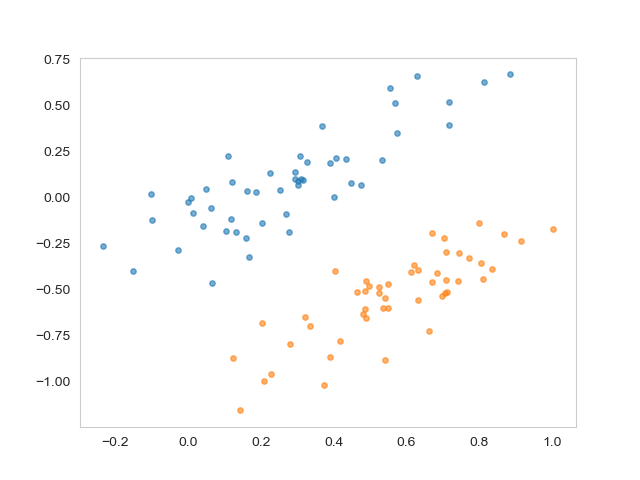
\includegraphics[width=7cm]{grafici/2blobs.png}
 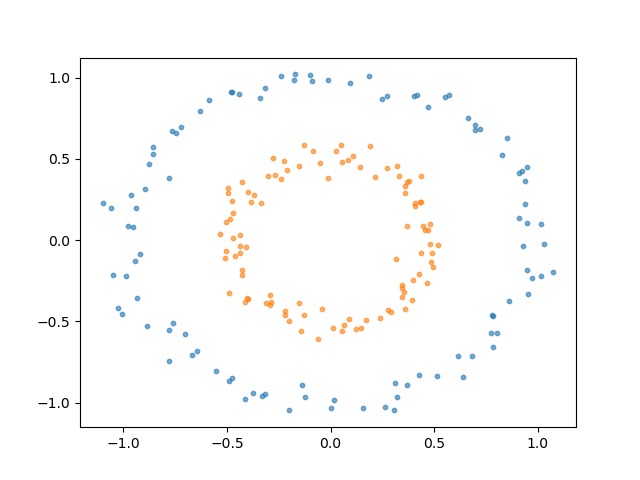
\includegraphics[width=7cm]{grafici/makecircles.png}
 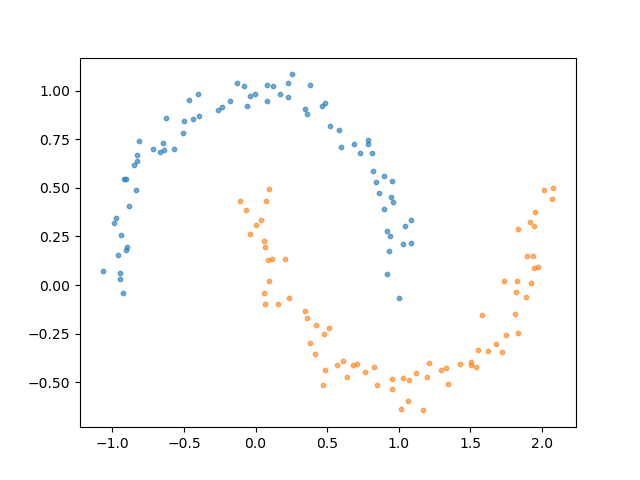
\includegraphics[width=7cm]{grafici/makemoons.png}        
\caption{\emph{\textbf{blobs}}, \emph{\textbf{circles}} and \emph{\textbf{moons}} datasets.}
        \label{datasets}
    \end{figure}   



\newpage



\section{Clustering algorithm based on the Mondrian Process}


The tree structure of the Mondrian process, that reflects the way in which the Mondrian process partitions the space, naturally leads to its adaptation to a clustering hierarchical algorithm.
The adapted process differs from the pure Mondrian process because the split criterion must rely on some characteristic of the data that we want to cluster.


The Mondrian clustering algorithm consists of a two-step process.%\footnote{or three?}.
The first part  has a top-down approach and is the one that directly exploits the Mondrian process; 
it partitions the space on which the set of data is defined and, for each leaf node, assigns all the data belonging to the corresponding subspace to the same cluster.
The second part of the two-step process has a bottom-up approach;
it starts from considering each final subspace (corresponding to a leaf node of the tree) as an independent cluster and hierarchically merges them on the basis of the same metric used in the previous splitting process.




\subsection{Partitioning}


The partitioning of the space is the phase of the method that directly involves the adaptation of the Mondrian process.
The main differences from the pure Mondrian process are that both the definition of the initial space and the cut choice depend on the input unlabeled data $\pmb{X} = (\pmb{x}_1,...,\pmb{x}_n) \in \mathbb{R}^D$;
as regards the initial space, it is defined as the smaller axis-aligned box $\Theta$ that contains $\pmb{X}$.\\
Following the scheme presented in Section \ref{defMP}, the new data-dependent Mondrian recursive generative process is shown below:\\ \\ 
DATA-DEPENDENT-MONDRIAN($\pmb{X}$,$\Theta$,$t_0$):%\footnote{il fatto dei vicini forse non serve scriverlo adesso}
\begin{enumerate}[nolistsep]
\item $T \sim Exp$(vol($\Theta(\pmb{X}))))$  
\item h $\sim \{$hyperplane($\pmb{x}_i,\pmb{x}_j)$ with $p \propto p_{i,j} \lvert (\pmb{x}_i,\pmb{x}_j) \in \pmb{X}\}$
\item $\pmb{X}_<,\pmb{X}_>$ with $\pmb{X}_< \in \Theta_<$, $\pmb{X}_> \in \Theta_>$ and $\pmb{X}_< \cup \pmb{X}_> = \pmb{X}$, $\Theta_< \cup \Theta_> = \Theta$
\item $M_< \leftarrow$DATA-DEPENDENT-MONDRIAN($\pmb{X}_<,\Theta_<,t_0+T$) 
\item $M_> \leftarrow$ DATA-DEPENDENT-MONDRIAN($\pmb{X}_>,\Theta_>,t_0+T$) 
\end{enumerate}
return ($t_0+T,h,M_<,M_>$)\\ \\%t_0,\Theta_<,\Theta_>,
Firstly, the time of the cut is generated from an exponential distribution with rate the volume of the initial space (line 1);
this means that, as in the pure Mondrian process, the cut is expected to be sooner in larger boxes than in smaller ones.
Then, for each pair of points $\in \pmb{X}$, an hyperplane intersecting the space $\Theta$ is associated and a metric is calculated;
the metric $p_{i,j}$ defines the degree of similarity between the two subset of points separated by the corresponding hyperplane.
In line 2, the hyperplane of the cut is randomly generated from the ensemble of the hyperplanes that have been associated to each pair of data points, with probability of extraction proportional to the metric value.
In line 3, the two just separated subsets of points $\pmb{X}_<$ and $\pmb{X}_>$ are associated to the corresponding subspaces $\Theta_<$ and $\Theta_>$. 
As in the pure Mondrian process, in lines 4 and 5, the previous steps are independently repeated over the two new subspaces.

The whole process stops when, as in the pure Mondrian process, the absolute time $t_0+T$ is higher than $\lambda$, or when the set of data $\pmb{X}$ contains only two points.
The ensemble of the leafs of the Mondrian tree shows the final and more refined partition of the initial space and the union of all the sets of points contained in the leaf subspaces is equal to the initial set of data $\pmb{X}$.
All the data that are contained in the same subspace are considered to belong to the same cluster .


Figure \ref{partition} shows an example of one possible output of the partitioning phase run on \emph{\textbf{circles}} datasets. %and \emph{\textbf{moons}} datasets.
It is obtained by hierarchically splitting the initial space through 15 cuts and the final partition consists of 16 adjacent polygones.
Each subspace is associated to its characteristic number.


\begin{figure}[H]
        \centering
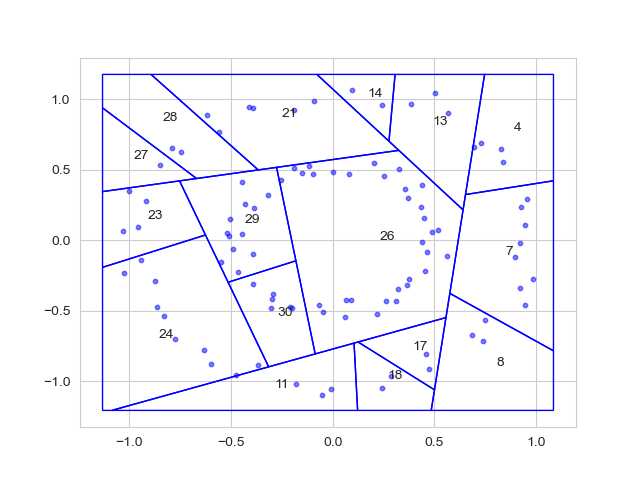
\includegraphics[width=8cm]{grafici/circles_partitioning.png}
\caption{Output of the partitioning phase run on \emph{\textbf{circles}} datasets}
\label{partition}
    \end{figure}   





\subsection*{Hyperplane and metric choice}

We considered three different choices for the hyperplane and the metric, that respectively are associated to each pair of points and estimates the similarity of two groups of data.
While how they are calculated is explained in the following, the differences between the three methods are highlighted in Section \ref{section_examples}.

Since a way to estimate the similarity of two groups of data is to evaluate how they are spatially separated, the chosen metrics are functions of the euclidean distance;
in particular, the minimum distance between and within the two groups of data are compared.

Lower is the value of the metric, more similar are the two groups of points;
for this reason this value can be used as probability of extraction of the corresponding cut (higher is the value of the metric, less similar are the two groups of data and higher is the probability to extract the hyperplane).
%Remind that $\pmb{X}$ is a $D$-dimensional set of data.





\paragraph{Algorithm 1}
%Axis-aligned hyperplanes and metric 1}

In this first case, we don't associate an hyperplane to each pair of points $\in \pmb{X}$  but we consider their projections on the coordinate axis.
For each dimension, an hyperplane is thus associated to each pair of consecutive projections;
it is orthogonal to the corresponding $d$ coordinate axis (as in the pure Mondrian process) and intersects the segment connecting the two projection points in its middle point.
%If $n$ is the number of data points,we have a set of $(n-1) \cdot d$ possible hyperplanes. 






The metric is calculated according to the following scheme:\\ \\
METRIC($\pmb{X}_<$,$\pmb{X}_>$):
\begin{enumerate}[nolistsep]
\item $d_{min}$ = min(\emph{dist}($\pmb{X}_<$,$\pmb{X}_>$))\\
calculate the minimum distance between points belonging to the two different subspaces (\emph{dist} is the euclidean distance)
\item $d_i$ = min(\emph{dist}$(\pmb{x}_i,\pmb{X}_j)$ $\forall \pmb{x}_i \in \pmb{X}_j$ where $j=<,>$ \\
for each point in $\pmb{X}_<$ and $\pmb{X}_>$, calculate the minimum distance between the considered point and an other point of the same group
\item $\bar{d} = (\sum_{i=1}^D d_i)/D$ \\
 calculate the mean of the minimum distances within the groups (calculated in line 2)
\item $\emph{metric} = \lvert d_{min} - \bar{d} \lvert$\\
the metric is the absolute value of the difference between the minimum distance between the groups and the mean of the minimum distances within the groups
\end{enumerate}
return($\emph{metric}$)\\ \\





\paragraph{Algorithm 2}
%Non-axis-aligned hyperplanes and metric 1}
Here the metric is the same of the previous case, while the way to generate the hyperplanes is changed:
the cuts are no more linked to be orthogonal to the coordinate axis, but can in principle take any direction of the space.
For each pair of points, an hyperplane is associated: 
it is orthogonal to the segment connecting the two points and intersects it in its middle point.




\paragraph{Algorithm 3}
%Non-axis-aligned hyperplanes and metric 2}
In this third considered procedure, the hyperplanes can take any direction and are generated as in the previous case.
The metric is instead lightly changed (see Figure \ref{metric} for a visualization of the considered segments):\\ \\
METRIC-WITH-CORRECTION($\pmb{X}_<$,$\pmb{X}_>$):
\begin{enumerate}[nolistsep]
\item $d_{min}$ = min(\emph{dist}($\pmb{X}_<$,$\pmb{X}_>$))\\
calculate the minimum distance between points belonging to the two different subspaces (\emph{dist} is the euclidean distance);
we call the nearest pair $(\pmb{x}_{<,1},\pmb{x}_{>,1}) \in \pmb{X}_< \times \pmb{X}_>$ 
\item $d_i$ = min(\emph{dist}$(\pmb{x}_i,\pmb{X}_j)$ $\forall \pmb{x}_i \in \pmb{X}_j$ where $j=<,>$ \\
for each point in $\pmb{X}_<$ and $\pmb{X}_>$, calculate the minimum distance between the considered point and an other point of the same group
\item $\bar{d} = (\sum_{i=1}^D d_i)/D$ \\
 calculate the mean of the minimum distances within the groups (calculated in line 2)
\item $d_{min,<}$ = min(\emph{dist}($\pmb{x}_{<,2}$,$\pmb{X}_>$))\\ 
consider $\pmb{x}_{<,2}$, the nearest point to $\pmb{x}_{<,1}$ belonging to $\pmb{X}_<$; 
calculate the minimum distance between $\pmb{x}_{<,2}$ and a point belonging to $ \pmb{X}_>$
\item $d_{min,>}$ = min(\emph{dist}($\pmb{x}_{>,2}$,$\pmb{X}_<$))\\ 
consider $\pmb{x}_{>,2}$, the nearest point to $\pmb{x}_{>,1}$ belonging to $\pmb{X}_>$; 
calculate the minimum distance between $\pmb{x}_{>,2}$ and a point belonging to $ \pmb{X}_<$
\item $\emph{metric} = \lvert d_{min} - \bar{d} \lvert + d_{min,<} + d_{min,>}$
\end{enumerate}
return($\emph{metric}$)\\ \\





\begin{figure}[H]
        \centering
        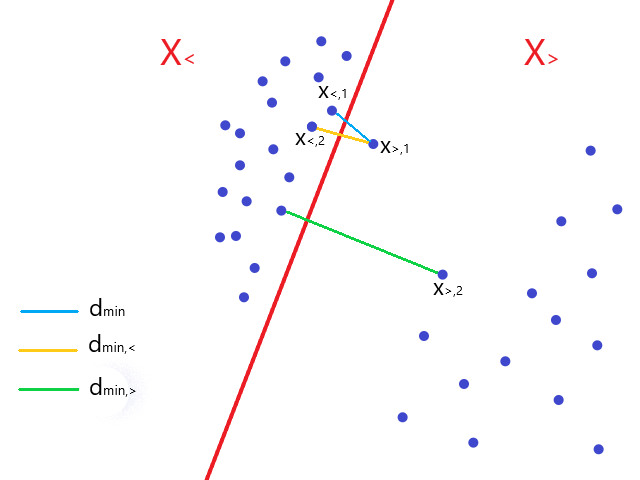
\includegraphics[width=8cm]{grafici/METRIC2.png}
\caption{Points and segments considered in the calculation of the metric; $\pmb{X}_<$ and $\pmb{X}_>$ are the two sets of data separated by the red line. }
\label{metric}
    \end{figure}   



\subsubsection*{Mathematical description}


\paragraph{Hyperplane} 

If we consider a $D$-dimensional space $\Theta$, an hyperplane is a $(D-1)$-dimensional subspace of $\Theta$.
It can be described by a linear equation $a_1 x_1 + ... + a_{D-1} x_{D-1} = b$ or by a radius vector orthogonal to it;
from a computational point of view, the description through the normal vector is more convenient, since it is more easily generalized to generic dimensions. 
In particular, each hyperplane is characterized by a set of $D-1$ point coordinates, that univocally determine the direction of the normal vector, and a scalar, representing its magnitude (that is the distance between the hyperplane and the origin of the axes).

\paragraph{Polytope}
While, if we consider only axis-aligned cuts, the generated subspaces are all axis-aligned boxes, in case of cuts with generic directions, the subspaces are no more cartesian products of boundend intervals but are generic convex polytopes (the convexity property holds if the initial space is convex).
A polytope is mathematically described through its \emph{half-space representation}, that means it is defined by intersection of a finite number of half spaces.
In particular, starting from the equation of the hyperplane that splits the whole space into two half spaces, we can write each linear half space as linear inequality: $a_1 x_1 + ... + a_{D-1} x_{D-1} \leq b$ and $a_1 x_1 + ... + a_{D-1} x_{D-1} \geq b$.
A polytope is thus described as a system of linear inequalities, and the number of the inequalities is equal to the number of sides of the polytope:\\
$a_{1,1} x_1 + ... + a_{1,D-1} x_{D-1} \leq b_1$\\
$a_{2,1} x_1 + ... + a_{2,D-1} x_{D-1} \leq b_2$\\
     $\cdots$  \\
$a_{m,1} x_1 + ... + a_{m,D-1} x_{D-1} \leq b_m$\\
The system of inequalities can be written in matrix form $\bf{A} \cdot \bf{x} = \bf{b}$;
a polytope is thus characterized by a $m \times (D-1)$ matrix \textbf{A} and a $m$-dimensional vector \textbf{b}.



\subsection{Merging}

While the first part of the algorithm partitions the space and separates the data into several groups, the second part collects the subspaces into clusters and assigns them to different classes.
%Once the space has been partitioned and the data have been separated into several groups, the
%the scope of the second part of the algorithm is to group the different subspaces

%The similarity criterion used to gather neighbouring subspaces, in order to find which of them belong to the same class,  is the same metric used to partition the space in the first part of the algorithm and is described in eccecc.
%thus depends on some function of the distance between data.
%The metric is calculated for each pair of adjacent polytopes.

A bottom up approach is used; this means that, firstly, no more than one subspace is assigned to the same class and thus the number of classes is equal to the number of subspaces (remind that all the points belonging to the same subspace belong to the same class).
The initial state is described by an undirected network $G$ with number of nodes equal to the number of subspaces and without edges.
Then, edges are progressively added to the network.
%The, pair of neighbouring subspaces are progressively merged by adding
The presence of an edge connecting two nodes means that two subspaces are merged, consequently assigning the corresponding groups of data to the same class;
this means that, at each step, the total number of classes is equal to the number of connected components of the network.
The order in which the edges are added to the network is determined by assigning a score to each edge;
it represents a similarity measure between groups of data and is the same metric %, described in eccecc, 
used to partition the space in the first part of the algorithm.
The lower is the value of the metric, more similar are the two groups of data contained in neighbouring subspaces and more likely are the subspaces to belong to the same class.
After the scores of all the possible edges are calculated, the edge with lower score is added to the network and the two subspaces corresponding to the nodes linked by the edge are merged;
the metric is thus again calculated for the pairs of neighbouring subspaces and the score list is updated.
Only edges that connect adjacent polytopes are considered.



Because both the metrics METRIC and METRIC-WITH-CORRECTION can't be calculated if one of the two subspaces contains single data, before creating the network $G$, each subspace with single data is merged to the corresponding nearest neighbouring subspace containing more than one data.
More precisely, if $\pmb{x}_1$ is the data contained in the single-data partition and $\pmb{X}_2$ is the set of data contained in the second subspace, the closeness between two adjacent subspaces is determined by the following metric:\\ \\
METRIC-SINGLE-DATA($\pmb{x}_1$,$\pmb{X}_2$):
\begin{enumerate}[nolistsep]
\item $d_{min,1}$ = min(\emph{dist}($\pmb{x}_1$,$\pmb{X}_2$))\\ 
calculate the distance between $\pmb{x}_1$ and its nearest point belonging to $\pmb{X}_2$;  we call it $\pmb{x}_{2,1}$
\item $\pmb{x}_{2,2} \in \pmb{X}_{2}$\\
find the nearest point to $\pmb{x}_{2,1}$ belonging to $\pmb{X}_{2}$
\item $d_{min,2}$ = \emph{dist}($\pmb{x}_{1},\pmb{x}_{2,2}$))\\ 
calculate the distance between $\pmb{x}_{2,2}$ and $\pmb{x}_1$; 
\item \emph{metric} =  $d_{min,1} + d_{min,2}$
\end{enumerate}
return(\emph{metric})\\ \\
%\footnote{devi spiegare perchè hai scelto questa metrica e nn la semplice distanza minima. allora devi spiegare anche per le altre metriche appena dopo lo schema e non quando fai l'esempio}\footnote{forse usare questa metrica è un po' inutile. basterebbe sommare le due distanze minime dal singolo punto}\footnote{due partizioni con dati singoli non vengono unite perchè altrimenti cambiaerebbe la metrica. in realtà questo non va tanto bene, l'ho messo solo per semplicità}

Figure \ref{merging} shows three steps of the merging process applied to a partition of \emph{\textbf{blobs}} dataset. 
On the left, the partitioned space is shown, with the subspaces belonging to the same class characterized by the same color;
the total number of colors is equal to the number of connected components of the corresponding network, shown on the right.


\begin{figure}[H]
        \centering
        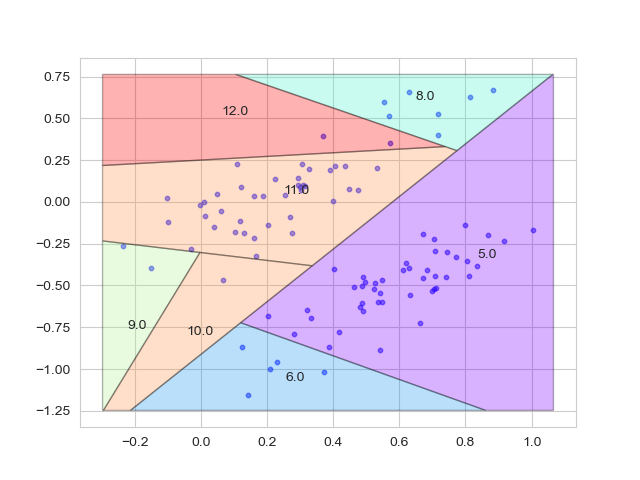
\includegraphics[width=8cm]{grafici/2blobs_4_6.png}      
        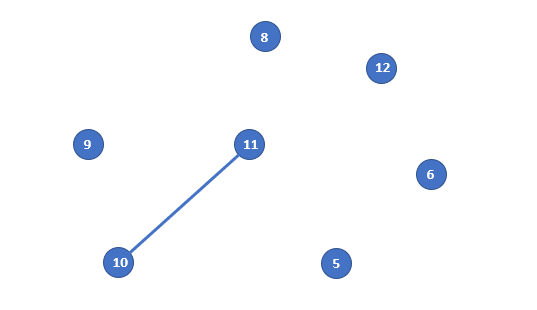
\includegraphics[width=8cm]{grafici/2blobs_4_6_G.png}      
        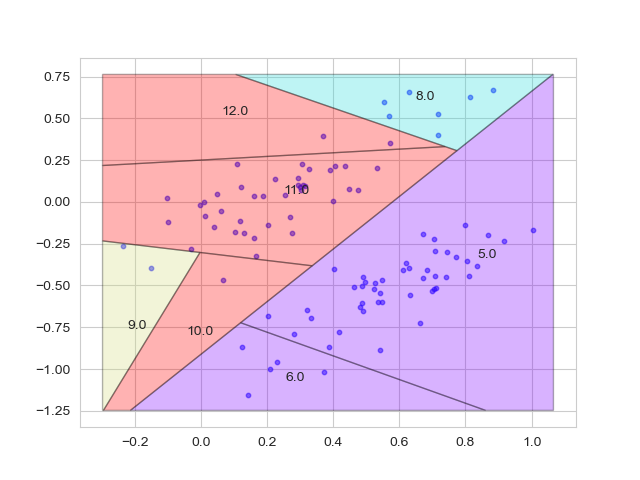
\includegraphics[width=8cm]{grafici/2blobs_4_4.png}      
        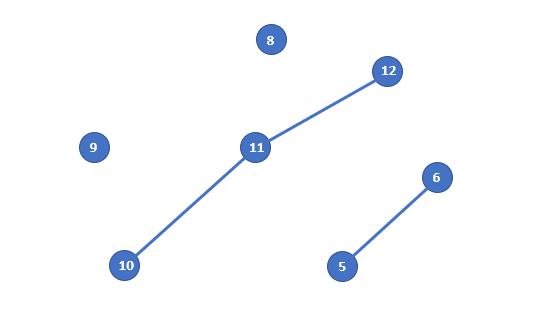
\includegraphics[width=8cm]{grafici/2blobs_4_4_G.png}      
        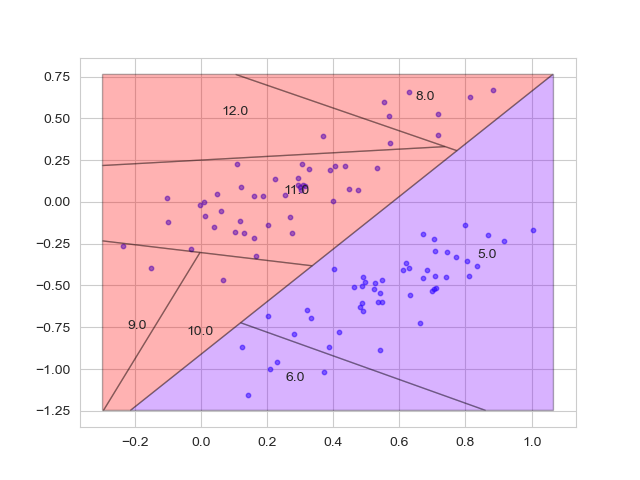
\includegraphics[width=8cm]{grafici/2blobs_4_2.png}      
        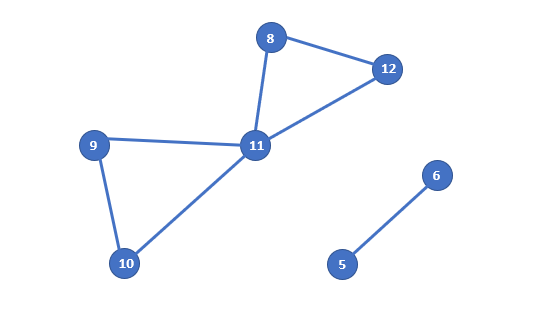
\includegraphics[width=8cm]{grafici/2blobs_4_2_G.png} 
\caption{Three steps of merging process with corresponding graphs}
        \label{merging}
    \end{figure}   


\newpage
\section{Mondrian clustering forest}


The output of the merging process doesn't give us information about how many clusters characterize the dataset.
In fact, it considers different cases, each one characterized by a fixed number of clusters;
for each case, it estimates how the subspaces are clustered, but is not able to determine what is the most probable among them.
In order to automatically determine the number of clusters, a Mondrian clustering forest is considered;
it is the equivalent of an unsupervised random forest based on Mondrian clustering algorithm.

The main advantage of the forest is that its output associates, to each point of the space, a measure of the probability to belong to a certain class.
Figure \ref{forest} shows, on the left, a visualization of the averaged output of 10 Mondrian trees in case of \emph{\textbf{moons}} dataset.
The region characterized by a lighter color has a probability $p_1 = 1$ to belong to the first class and a probability $p_2 = 0$ to belong to the second class;
on the contrary, the darker region has $p_1 = 0$ and $p_2 = 1$.
The regions characterized by a range of intensities between the lighter and the darker ones are associated to different values of probabilities in the interval $[0,1]$ without extremes.

Moreover, the forest allows us to automatically determine the number of clusters in which the data and the corresponding space are divided.
For this purpose, we consider, for each tree, the labeling associated to each point of the dataset, obtained by the merging procedure of the algorithm;
for each possible number of cluster, we have a different set of labeled data.
The labels obtained by two different trees are compared, through the \emph{adjusted mutual information} score, for each possible fixed number of clusters, and this measure is repeated for each possible pair of considered trees.
The \emph{adjusted mutual information (AMI)} \cite{scikit-learn} is a function of the entropy of the two different partitions of the same set of data;
it quantify the information shared by the two partitions and is thus a measure of the similarity of two labeling of the same set of data, ignoring permutations.
It ranges between 0 and 1 and higher is its value, more similar are the two set of labels.
Figure \ref{forest}, on the right, shows a plot of the \emph{adjusted mutual information} score in function of the number of clusters;
each line corresponds to a specific pair of tree outputs;
all the values of the score (corresponding to different pairs of trees) are averaged, for each fixed number of clusters, and the mean value is represented by the more intense blue dotted line.
At this point, the number of clusters corresponding to the higher value of the \emph{AMI} score is considered the most probable.
The plot of \emph{AMI} score vs the number of clusters in Figure \ref{forest} is referred to the forest of 10 Mondrian trees applied to \emph{\textbf{moons}} dataset;
the higher value of compatibility between tree is obtained for the number of clusters equal to 2.



\begin{figure}[H]
        \centering
        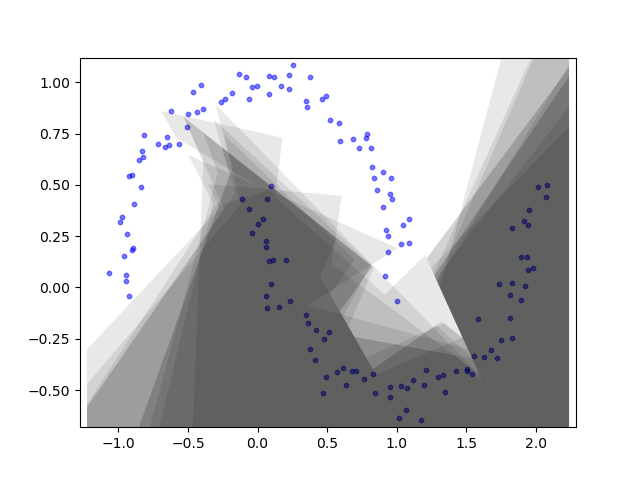
\includegraphics[width=8cm]{grafici/moons_plot_binario.png}      
        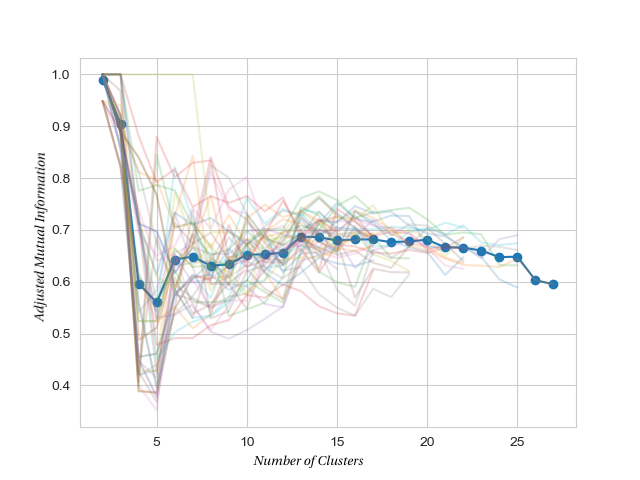
\includegraphics[width=8cm]{grafici/makemoons_2_escluso1_2.png}   
\caption{On the left, the output of a Mondrian clustering forest applied on \emph{\textbf{moons}} dataset; on the right, the corresponding plot of \emph{AMI} score vs number of clusters.}
        \label{forest}
    \end{figure}   



\newpage
\section{Examples in 2D}\label{section_examples}




In the next sections, some example are shown, in order to clarify the performance of the algorithm, the differences of the three versions and to highlight some numeric issues related to methodological choices






\subsection{Algorithm 1 vs Algorithm 2: evaluation of \emph{partitioning} phase}

In this section we consider the two versions of the algorithm characterized by different choices of the hyperplanes and the same similarity criterion METRIC.

Figures \ref{blobs_1vs2} and \ref{circles_1vs2} show the partitioning phase of \textbf{Algorithm 1} and \textbf{Algorithm 2}, applied to datasets \emph{\textbf{blobs}} and \emph{\textbf{circles}}.
In order to evaluate the result of partitioning phase, we can firstly check if each final subspace contains only data belonging to the same class;
moreover, since the number of splits is related to the computational cost of the algorithm, we can measure how many splits are necessary to completely separate the two clusters.

In each of the four considered cases, the space is splitted in order to have each polygon containing data belonging only to one class;
from this point of view, it means that the two methods are equivalent and the partitioning output of both the algorithms can be considered a good input for the next \emph{merging} phase.

As regards the evaluation of computational costs, consider Figure \ref{blobs_1vs2}.
While, in the partitioning procedure performed by \textbf{Algorithm 2}, the first split is enough to totally separate the two groups of data, in the other case the complete separation is obtained after nine splits;
this means that the method with cuts that are not linked to be orthogonal to the coordinate axis is much more convenient from a computational point of view, especially when the datasets require a splitting procedure on the diagonal direction.

An other reason to prefer the non-axis-aligned cuts is the absence of preferred directions.
Figure \ref{circles_1vs2} shows \emph{\textbf{circles}} dataset, that is rotation-invariant with respect to the axis perpendicular to the plane and intersecting the center of the circles.
If we run several times \textbf{Algorithm 1} on the dataset, the cuts separating the two circles will be almost the same, because they are forced to be orthogonal to the axis;
on the contrary, the output of \textbf{Algorithm 2} shown in the figure is only a possible realization of the algorithm:
since the cuts can in principle take any direction and the process is randomized, different runs of the process give subspaces that contain the smaller circle with different shape.
The absence of preferred directions is important especially when considering the outcome of the Mondrian forest:
if we average several outputs of \textbf{Algorithm 2} trees, the probability distribution to belong to a certain class will reflect the rotation-invariance of the data, while in the other case the regions corresponding to different classes will be sharp-bordered and will show a presence of preferred direction that is not a real characteristic of the data.



%makecirclesorthogonal 81 splitslifetime=2
%2blobs 55 splits   lifetime=7




\begin{figure}[H]
        \centering
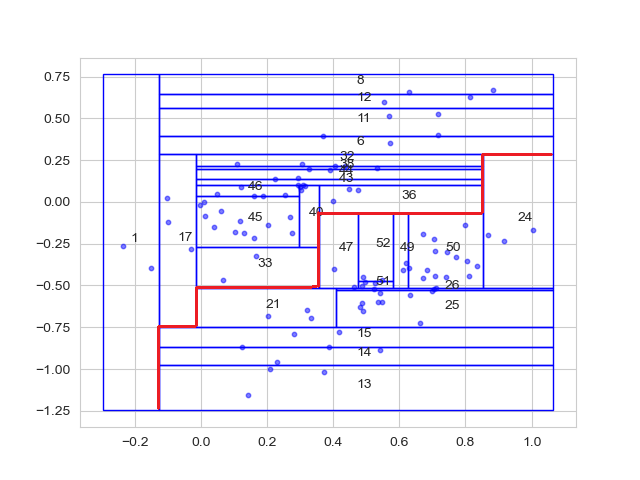
\includegraphics[width=8cm]{grafici/2blobs_alg1_2+.png}
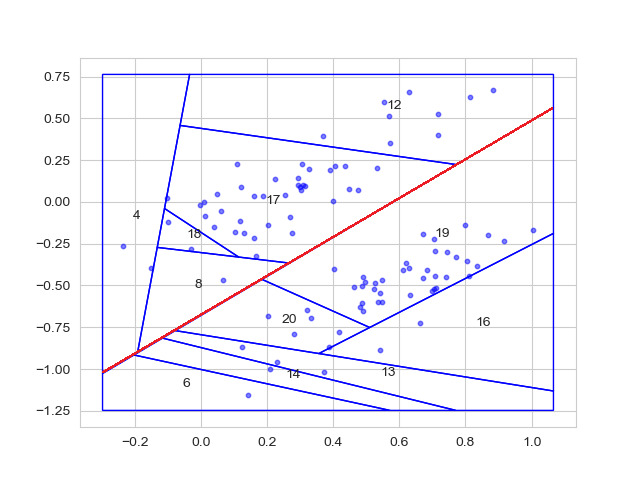
\includegraphics[width=8cm]{grafici/2blobs_alg2_2.png}
\caption{Plot of the final result of \emph{partitioning} phase (the subspaces are all leaf of the corresponding tree), applied to the datasets \emph{\textbf{blobs}}. The splitting criterion is determined by \textbf{Algorithm 1} at the left and \textbf{Algorithm 2} at the right.}
        \label{blobs_1vs2}
    \end{figure}   
\begin{figure}[H]
        \centering
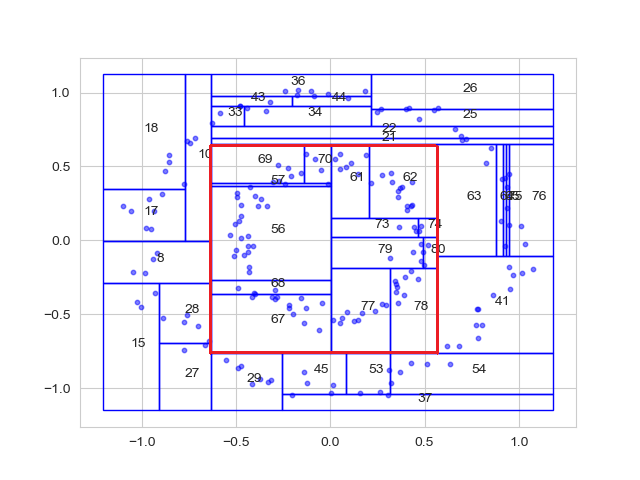
\includegraphics[width=8cm]{grafici/makecircles_alg1_2.png}
 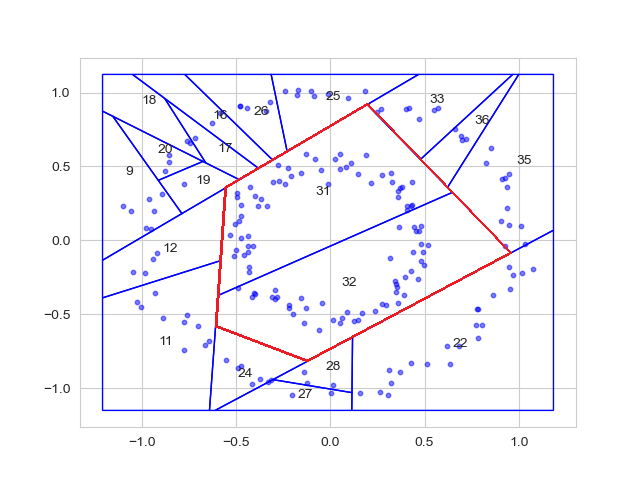
\includegraphics[width=8cm]{grafici/makecircles_alg2_2.png}
\caption{Plot of the final result of \emph{partitioning} phase (the subspaces are all leaf of the corresponding tree), applied to the datasets \emph{\textbf{circles}}. The splitting criterion is determined by \textbf{Algorithm 1} at the left and \textbf{Algorithm 2} at the right.}
        \label{circles_1vs2}
    \end{figure}

\begin{comment}
\begin{figure}[H]
\centering
\subfigure[q]
{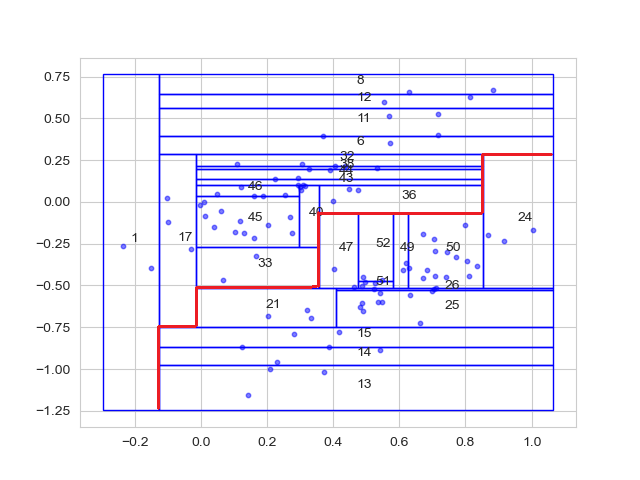
\includegraphics[width=8cm]{grafici/2blobs_alg1_2+.png}\label{blobs1}}
\subfigure[q]
{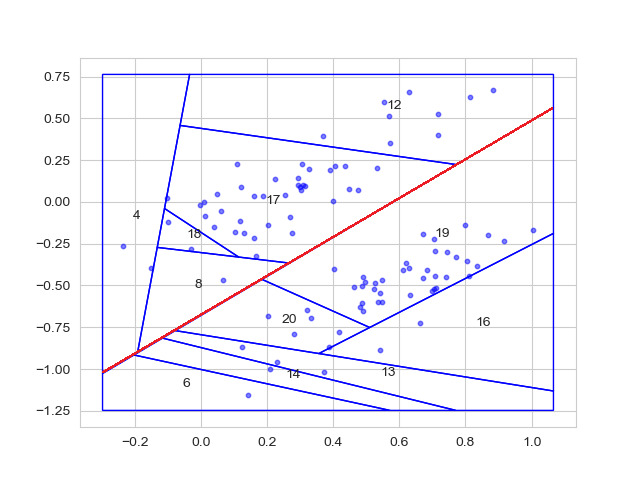
\includegraphics[width=8cm]{grafici/2blobs_alg2_2.png}\label{blobs2}}
\subfigure[q]
{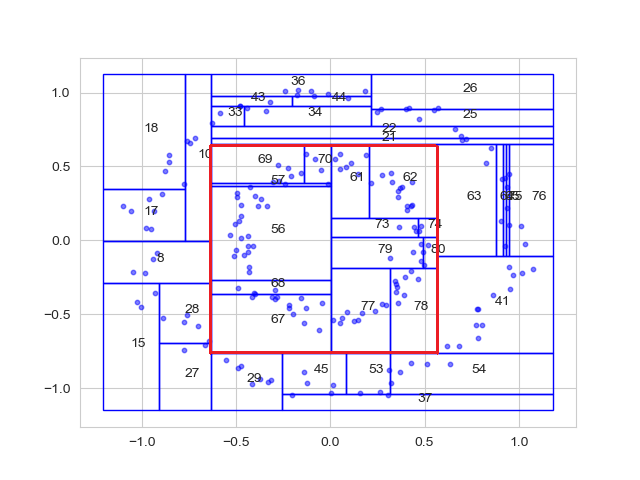
\includegraphics[width=8cm]{grafici/makecircles_alg1_2.png}\label{circles1}}
\subfigure[q]
{ 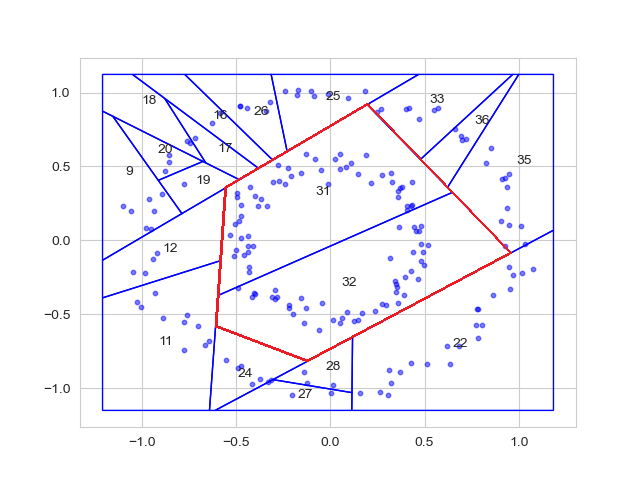
\includegraphics[width=8cm]{grafici/makecircles_alg2_2.png}\label{circles2}}
\caption{Evolution dynamics of the system defined by.}
\label{Coop}
\end{figure}
\end{comment}



\subsection{Algorithm 2 vs Algorithm 3: evaluation of \emph{merging} phase}

Here we compare the merging procedures obtained by employing the two different metrics starting from the same output of partitioning phase.
Figures \ref{2vs3} shows a space partition of \emph{\textbf{moons}} dataset that don't completely separate the two groups of data;
in particular, the subspace 14 contains one point belonging to the lower semicircle and all the other points belonging to the upper one.
If the groups of data are not well divided by the partitioning procedure, meaning that some final subspace contains points belonging to more than one class, we need the correction of the second metric (\textbf{Algorithm 3}) to better assign the clusters.

The left plot of Figure \ref{2vs3} shows the output of the merging procedure with \textbf{Algorithm 2} for 2 number of clusters:
by only considering the difference between the minimun distance between subspaces and the mean of the minimum distances within the subspaces (what METRIC does), the subspaces 14 and 10 are considered more similar than the subspaces 11 and 17 and, consequently, they are separated later;
we see that, in this case, the division into two cluster doesn't correspond to the division into two semicircles.

If we add the correction to the metric (\textbf{Algorithm 3}), the score depends on more than one minimum distance between subspaces and it is thus a way to take into account the presence of outliers.
The right plot of Figure \ref{2vs3} shows the correct classification of the dataset.






\begin{figure}[H]
\centering
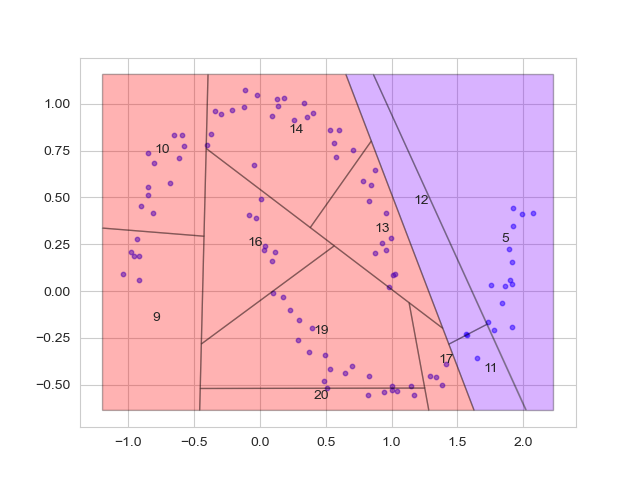
\includegraphics[width=8cm]{grafici/moons_2clusters_nocorr.png}
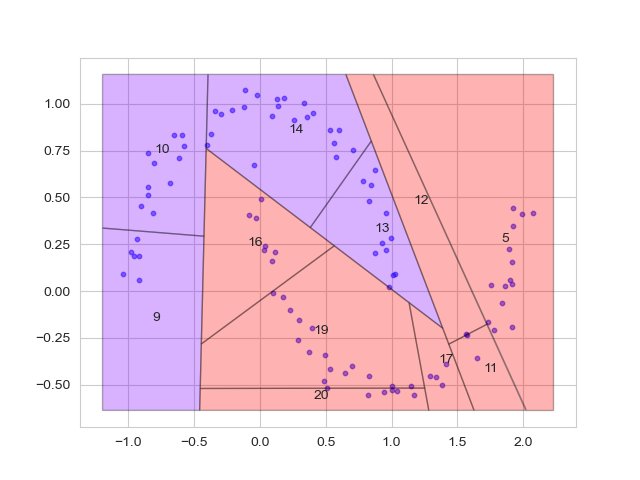
\includegraphics[width=8cm]{grafici/moons_2clusters_withcorr.png}
\caption{\emph{\textbf{moons}} dataset: merging process output for 2 clusters with METRIC (left) and METRIC-WITH-CORRECTION (right)}
\label{2vs3}
\end{figure} 

%\begin{figure}[H]
%\centering
%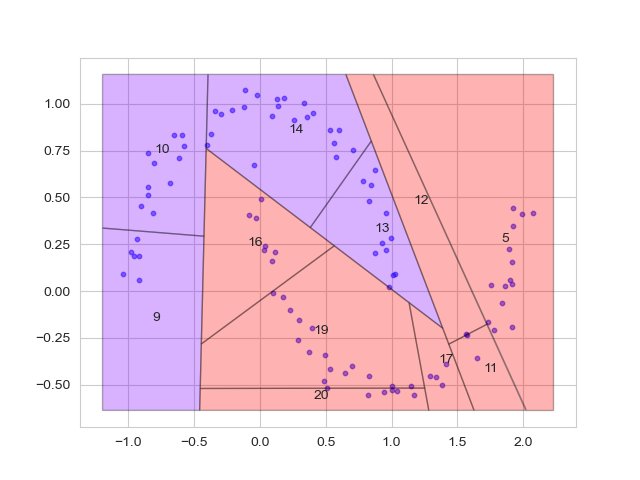
\includegraphics[width=8cm]{grafici/moons_2clusters_withcorr.png}
%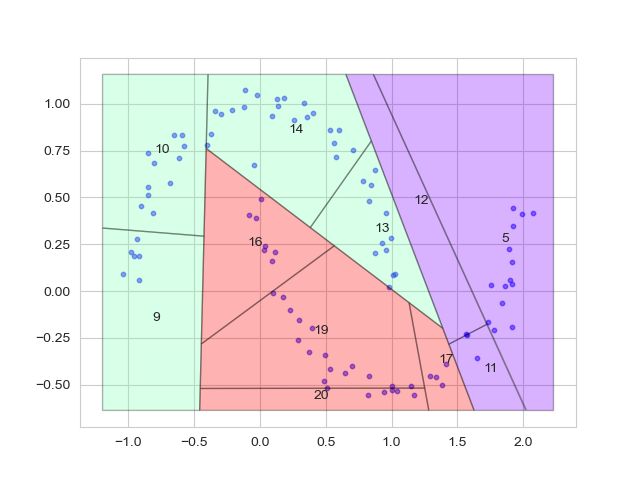
\includegraphics[width=8cm]{grafici/moons_3clusters_withcorr.png}
%\caption{\emph{\textbf{moons}} dataset: merging process output for 2 and 3 clusters with METRIC-WITH-CORRECTION}
%\label{withcorr_2vs3}
%\end{figure} 



\section{Conclusions}


The examples shown in this report suggest that a clustering algorithm based on the Mondrian process has some interesting aspects that it is worth to deeply investigate;
some of these are the fact that the output of the algorithm is a probability distribution that estimates how likely each data is to belong to a certain cluster, the automatic determination of the number of clusters and the absence of preferred directions in phase of space partitioning.
Some of the aspects that need to be explored are the following:
firstly, other toy datasets should be used, in order to verify if the algorithm works with any distribution of data in terms of shape and point density;
in particular, despite the code is written in order to work with generic dimension datasets, it is not obvious to obtain a good performance with more than 2-dimensional data.
Moreover, it may be possible that, even when the unsupervised classification provides good results, the automatic determination of the number of clusters doesn't work.
An other aspect that needs to be further studied is the role of the lifetime lambda and, in particular, how the complexity of the tree is related to the complexity of the dataset;
this means that it may be possible to know, before performing the classification, how many splits are necessary to well classify the dataset.
Finally, other alternatives to the formulation of the metric and the choice of the hyperplane should be find.


\begin{comment}
qual è ruolo di lambda?
\footnote{
scrivi da dove vengono i datasets e scrivi librerie usate nel codice
metti schemi in metrica (disegni)
}

%\section{extension in general dimensions}

We associate a metric value, calculated as in blablabla, to each possible cut and we use these values, raised to a certain power $e$, as probabilities for the random extraction of the hyperplane that we will use to divide the underlying space into two subspaces.
%Once the hyperplane is randomly extracted with probability proportional to the corresponding metric value, the underlying space is divided into two subspaces over which the entire process can be independently repeated.

in queto caso tutti i sottospazi snono axis aligne boxes 
convex polytipe
each leaf subspace is a convex polytope that contains a subset of $\pmb{X}$.



%sviluppa ed illustra le proprietà e le caratteristiche del processo di Mondrian utilizzato come classificatore: 
%perchè funziona, 
%come si implementa e 
%le problematiche numeriche connesse alla metodologia con un esempio di applicazione
%AGGIUNTA ESPONENTE
%DISTANZA CON MINIMI SEMPLICE
%DISTANZA MODIFICATA 
%RUOLO DI LAMBDA

come creare spazio iniziale (axis-aligned box oppure convex polytope?)
tempo da esponenziale con rate inverso del volume ha senso?
\footnote{lambda complexity of the tree}


\footnote{puoi spiegare qui perchè hai considerato questi casi oppure lo fai dopo con gli esempi (perchè tagli casuali è meglio di tagli perpendicolari e quindi seconda metrica è stata provata solo su tagli as direzione casuale)}

%\footnote{devi spiegare perchè hai scelto questa metrica e nn la semplice distanza minima. allora devi spiegare anche per le altre metriche appena dopo lo schema e non quando fai l'esempio}\footnote{forse usare questa metrica è un po' inutile. basterebbe sommare le due distanze minime dal singolo punto}\footnote{due partizioni con dati singoli non vengono unite perchè altrimenti cambiaerebbe la metrica. in realtà questo non va tanto bene, l'ho messo solo per semplicità}




%\subsection{problema dell'esponente}
spiega direttamnete per tagli non perpendicolari


\footnote{da verificare se determinazione automatica numero di cluster funziona anche con altri datasets e con diverso numero di classi}





\section{variare variabili}
esponente, lifetime, criterio cut(???)
\section{confronto mondrian con altri metodi di clustering}
dovresti trovare qualche modo per confrontarli



\subsubsection{tagli non perpendicolari}
vantaggio dei tagli non perpendicolari
puoi mostrare cinfronto fra mondrian con tagli perpendicolari e altro

\subsubsection{polytopes}
come sono definiti matematicamente

fai considerazione che tutte le partizioni sono concave
\subsubsection{criterio per decidere il cut}
confronto varianza e centroide lo metti?



\paragraph{scaletta}


\begin{enumerate}
\item definizione processo di mondrian
\item proprietà matematiche
\item ...
\item confronto mondrian con altri metodi di clustering
\item 


\end{enumerate}


preprocessign=togliere doppioni


The distinguishing feature of this recursive stochastic process is that it assigns  probabilities to the various events in such a way that it is consistent (in a sense we make precise
later). The implication of consistency is that we can extend the Mondrian process to infinite spaces
and use it as a nonparametric prior for modeling exchangeable relational data.
3.1 The one dimensional case
The







\paragraph{questioni}

\begin{enumerate}

\item decision tree non ha come output una probabilità
\item bayesian tree si
\item mondrian tree è una via di mezzo (si parla di tree o forest?)
\item exchangeable relational data


\end{enumerate}







\section{state of art}


My thesis work is about the development of a clustering method based on the Mondrian process.

The Mondrian process is a temporal stochastic process that randomly partitions the underlying product space in a hierarchical way, through axis-aligned cuts.% it has been discovered by jkdnakjbv in 2008

It is defined over a space that is a D-dimesional axis-aligned box theta, that means that each dimension of theta is a bounded interval.
The process is initialized by fixing the starting time t0 and the lifetime lambda.
Here is the scheme of the process that shows how the box theta is hierarchically cut in several subspaces:
firstly, the time of the first cut is randomly generated, from an exponential distribution with rate the linear dimension of theta; the linear dimension is a measure of the volume of the box and this means that the cut is expected to occur sooner in larger boxes that in smaller ones.
secondly, the dimension and the location of the cut are randomly generated: the dimension from a discrete distribution, with probability proportional to the lenght pf the intervals in each dimension: 
after generating the dimension of the cut, the location is generated uniformly in the interval and the cut is the hyperplane that intersect the space in that location and is orthogonal to the d dimension.

At this point, the initial space has been divided into two subspaces that are axis-aligned boxes as well and steps 1, 2 and 3 can be independently repeated over these two boxes with starting time t0+T

the process stops when the absolute time is higher than lambda.


here is an example of the mondrian process in 2 dimensions. in this case the initial space theta is a square with intervals defined from 0 to 1
the cut is always orthogonal to the generated dimension. in general, the cut is expected to intersect the larger dimension of the box. 
the space theta has been divided into two subspaces theta1 and theta2 and the process is independently repeated over these new boxes

As we can see from the left scheme, the Mondrian process has a binary tree structure, where each node represents a particular subspace of the initial box theta.                                                                                                                            
each internal node has always two children and the ensemble of the leaf nodes represents the final and more refined partition of the space.
( more deep is the tree, more refined is the partitioning of the product space.)


se vuoi qui puoi dire le propirietaà del mondrian process consistency ecc ecc


this is the pure mondrian stochastic process, now we see how it is used in machine learning.
The hierarchical tree structure of the mondrian process is a natural candidate for the partition structure of random decision trees
scrivi vantanggi di mondrian tree rispoetto a random tree 


noi però lo volgiamo usare per il clustering
dire breveììmente cosa è clustering 









\end{comment}




\nocite{*}

\printbibliography%[keyword={clustering}]














\begin{comment}




\subsection{Partitioning}


The partitioning of the space is the phase of the method that directly involves the adaptation of the Mondrian process.
The main differences from the pure Mondrian process are that both the definition of the initial space and the cut choice depend on the input unlabeled data $\pmb{X} = (\pmb{x}_1,...,\pmb{x}_n) \in \mathbb{R}^D$;
furthermore, the cut hyperplanes are no more axis-aligned but can take any direction.
as regards the initial space, it is defined as the smaller axis-aligned box that contains $\pmb{X}$, where $\pmb{X} = (\pmb{x}_1,...,\pmb{x}_n) \in \mathbb{R}^D$ is the set of input unlabeled data.
\footnote{veramente gli estremi non coincidono proprio con i dati più esterni, forse bisognerebbe impostarlo così?}\footnote{sarebbe effettivamente un po' più sensato ripensare allo spazio iniziale. la condizione è che deve essere convesso ma può non essere una axis-aligned box}


The process is initialized by fixing the initial time $t_0$ and the lifetime $\lambda$.


Firstly, the time of the cut is generated from an exponential distribution with rate the volume of the initial space\footnote{pensare};
this means that, as in the pure Mondrian process, the cut is expected to be sooner in larger boxes than in smaller ones.

Then, for each pair of points $\in \pmb{X}$, an hyperplane is associated; 
this hyperplane is orthogonal to the distance segment linking the two points and cuts the segment in its middle point.

The hyperplane of the cut is randomly generated from the ensemble of the hyperplanes that have been associated to each pair of data points.  
The probability of extraction of a particular hyperplane is proportional to a metric, representing the similarity between the two subsets of points separated by the cut. %belonging to the two subspaces of the initial box that are divided by the corresponding hyperplane;
we call the two subsets of data $\pmb{X}_1$ and $\pmb{X}_2$ and the calculation of the metric is described in the following scheme. \\ 
 
AssignMetric($\pmb{X}_1$,$\pmb{X}_2$):
\begin{enumerate}[nolistsep]
\item $d\_min$ = min(dist($\pmb{X}_1$,$\pmb{X}_2$)): calculate the minimum distance between points belonging to the two different subspaces; we call the nearest pair $(\pmb{x}_{1,1},\pmb{x}_{2,1}) \in \pmb{X}_1 \times \pmb{X}_2$; $dist$ is the euclidean distance.
\item for each point, calculate the minimum distance between the considered point and the other points of the same group; then take the mean $mean\_d\_min$ of the minimum values.
\item $d\_min_{1,2}$ = min(dist($\pmb{x}_{1,2}$,$\pmb{X}_2$)): consider $\pmb{x}_{1,2}$, the nearest point to $\pmb{x}_{1,1}$ belonging to $\pmb{X}_1$; 
calculate the minimum distance between $\pmb{x}_{1,2}$ and a point belonging to $ \pmb{X}_{2}$
\item $d\_min_{2,2}$ = min(dist($\pmb{x}_{2,2}$,$\pmb{X}_1$)): consider $\pmb{x}_{2,2}$, the nearest point to $\pmb{x}_{2,1}$ belonging to $\pmb{X}_2$; 
calculate the minimum distance between $\pmb{x}_{2,2}$ and a point belonging to $ \pmb{X}_{1}$
\item $metric = \lvert d\_min - mean\_d\_min \lvert + d\_min_{1,2} + d\_min_{2,2} $\\
\end{enumerate}

We associate a metric value, calculated as in blablabla, to each possible cut and we use these values, raised to a certain power $e$, as probabilities for the random extraction of the hyperplane that we will use to divide the underlying space into two subspaces.
%Once the hyperplane is randomly extracted with probability proportional to the corresponding metric value, the underlying space is divided into two subspaces over which the entire process can be independently repeated.
The previous steps are thus independently repeated over the two new subspaces.


The whole process stops when, as in the pure Mondrian process, the absolute time $t_0+T$ is higher than $\lambda$, or when the set of data $\pmb{X}$ contains only two points.

As the initial space is a convex polytope, anche le partizioni sono convesse

di qualcosa sul fatto che è un albero

The ensemble of the leafs of the Mondrian tree shows the final and more refined partition of the initial space;
each leaf subspace is a convex polytope that contains a subset of $\pmb{X}$.
All the data that are contained in the same polytope are considered to belong to the same cluster.
In the next phase the final subspaces are grouped and assigned to different classes.






%The scheme of the process is the following:\\
%%NOME( $\pmb{X}$,$t_0$,$\lambda$):
%\begin{enumerate}[nolistsep]
%\item $T \sim Exp(volume)$:  time of the cut
%\item cut hyperplane $\sim$ discrete(weights)
%\end{enumerate}
%come calcoli i pesi? altra fuznione




\subsection{unificazione partizioni}
 
While the first part of the algorithm partitions the space and separates the data into several groups, the second part collects the subspaces into groups and assign them to different classes.
%Once the space has been partitioned and the data have been separated into several groups, the
%the scope of the second part of the algorithm is to group the different subspaces

%The similarity criterion used to gather neighbouring subspaces, in order to find which of them belong to the same class,  is the same metric used to partition the space in the first part of the algorithm and is described in eccecc.
%thus depends on some function of the distance between data.
%The metric is calculated for each pair of adjacent polytopes.

A bottom up approach is used; this means that, firstly, no more than one subspace is assigned to the same class and thus the number of classes is equal to the number of subspaces.
The initial state is described by an undirected network $G$ with number of nodes equal to the number of subspaces and without edges.
Then, edges are progressively added to the network.
%The, pair of neighbouring subspaces are progressively merged by adding
The presence of an edge connecting two nodes means that two subspaces are merged, consequently assigning the corresponding groups of data to the same class;
this means that the total number of classes is equal to the number of connected components of the network.
The order in which the edges are added to the network is determined by assigning a score to each edge;
it represents a similarity measure between groups of data and is the same metric %, described in eccecc, 
used to partition the space in the first part of the algorithm.
The lower is the value of the metric, more similar are the two groups of data contained in neighbouring subspaces and more likely are the subspaces to belong to the same class.
After the scores of all the possible edges are calculated, the edge with lower score is added to the network and the two subspaces corresponding to the nodes linked by the edge are merged;
the metric is thus again calculated for the pairs of neighbouring subspaces and the score list is updated.
Only edges that connect adjacent polytopes are considered.



Because the metric defined in eccecc can't be calculated if one of the two subspaces contains single data, before creating the network $G$, each subspace with single data is merged to the corresponding nearest neighbouring subspace containing more than one data.
More precisely, if $\pmb{x}_1$ is the data contained in the first partition and $\pmb{X}_2$ is the set of data contained in the second one, the closeness between two adjacent subspaces is determined by the following metric:\\

MergePartitionssingledata($\pmb{x}_1$,$\pmb{X}_2$):
\begin{enumerate}[nolistsep]
\item $d\_min_1$ = min(dist($\pmb{x}_1$,$\pmb{X}_2$)): calculate the distance between $\pmb{x}_1$ and its nearest point belonging to $\pmb{X}_2$;  we call it $\pmb{x}_{2,1}$. ($dist$ is the euclidean distance)
\item $\pmb{x}_{2,2} \in \pmb{X}_{2}$: find the nearest point to $\pmb{x}_{2,1}$ belonging to $\pmb{X}_{2}$; 
\item $d\_min_2$ = dist($\pmb{x}_{1}$,$\pmb{x}_{2,2}$)): calculate the distance between $\pmb{x}_{2,2}$ and $\pmb{x}_1$; 
\item $metric =  d\_min_{1} + d\_min_{2} $\\
\end{enumerate}


\end{comment}







\end{document}




